
% !TeX encoding = utf8
% !TeX root = ./main.tex

% part I
% \titleformat{\chapter}
%   {\chap}{\thechapter}{1em}{}
% \titlespacing*{\chapter}{0pt}{3.5ex plus 1ex minus .2ex}{2.3ex plus .2ex}
%
\part{毕业论文}

% -------------------------------------------------------------------------
\chapter{引言}
% -------------------------------------------------------------------------

\section{研究背景与意义}

近年来,随着城市安防越来越被重视,安防监控系统越来越普及。
复杂的摄像头网络和海量的视频数据,使得依赖人力观察每个监控设备视频的方法不再适用。
智能行人监控技术应运而生,其中行人再识别(Person Re-identification, Person Re-ID)作为智能行人监控系统的核心技术之一,成为一个新的研究热点。
近几年,再识别领域投稿数量和性能均呈指数增长,
2015年性能指标CMC-1(Cumulative Matching Characteristic with Rank-1, 累计匹配特征曲线取第一个预测结果的准确率)
% todo cmc-1
只有$65\%$。17年达到了$80\%-85\%$。随后17年11月,在Arxiv上抢先公布的技术报告已经达到了$90\%-96\%$,号称在大型数据集上超越人类的表现。预计18年行人再识别领域的会有更多应用点和突破点。

图~\ref{fig:overall}为智能行人监控系统的系统框架。
总体上来说,智能行人监控系统应该被分解为三个子模块:行人检测(Pedestrian Detection),行人跟踪(Pedestrian Tracking),行人检索(Pedestrian Retrieval)。
其中行人检测是从视频监控视频每一帧中检测出行人的技术;行人跟踪是在时序上将行人串联起来形成视频片段的技术;
而行人检索是利用得到的行人图像完成跨摄像头行人检索的技术。
根据Zheng \etal \cite{zheng2017person}的定义,前两个模块是计算机视觉中已经存在的任务,因此大多研究者所指的行人再识别问题(Person Re-identification,Person Re-ID)着力解决第三个模块,也即
行人检索问题。
本文也不例外,着力解决光照、姿态、视角急剧变化下的行人再识别问题,也即行人检索问题。

\begin{figure}
	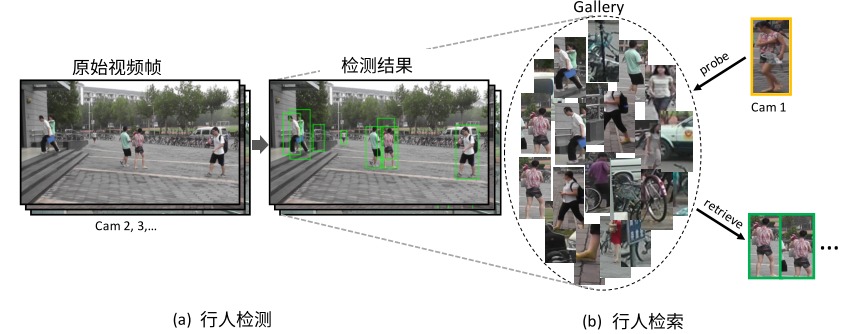
\includegraphics[width=\textwidth]{background.png}
	\caption{智能行人监控系统总体框架,图片修改自~\cite{zheng2017person}}
	\label{fig:overall}
\end{figure}

\section{国内外研究现状}

目前国内外行人再识别的研究主要集中在两方面的关键技术。
首先是提取具有鉴别能力的行人特征。
具有鉴别力的行人特征必须能够反映出行人个人的最基本特征,
同时也需要对环境的变化(包括相机视野不交叉导致的明暗变化和各种环境噪声,
行人刚性和非刚性变形导致姿态变化
)具有一定的鲁棒性;
其次是度量匹配空间的学习,
对于行人再识别任务,我们需要一个存在于统一嵌入空间的距离映射函数,
使得具有相同身份的行人图像距离尽可能小,一致性度量标准尽可能大,
同时最大化不同身份的行人图像距离,最小化一致性度量标准。

对于提取有鉴别能力的行人特征,先有的工作通常融合局部特征并引入注意力机制。
融合局部特征\cite{reciprocal},\cite{liu2017hydraplus},\cite{zhao2017spindle},\cite{glad}。比如,
Li \etal \cite{latent}使用STN结合先验定位可变性的行人部分,
从原始图片中预测定位参数,从而便于后续的网络将注意力集中于具有潜在语义的身体部分。
考虑到视频监控环境下行人的姿态先验——行人通常直立于地面,作者使用了4个自由度的仿射变换矩阵,建模了尺度、平移方面的可变性变换。
最终提取出更具语义特性的行人特征。

对于度量空间学习,由于行人再识别问题本身的特性,它的实际输入通常是一对图像或一个列表的图像,
然后在此基础上进行相似性度量或距离度量。
而我们知道,ImageNet时代大规模分类任务\cite{deng2009imagenet}
尽管取得了惊人的效果,
但是它相当于学习了每个类别的模板,只能保证已知类别图片的可分性,
这种方法在行人再识别问题上往往不再适用。
对此,国内外学者提出了大量
度量学习损失函数,包括对比损失(Contrastive loss)\cite{varior2016gated}、三元组损失(Triplet loss)\cite{schroff2015facenet}、四元组损失(Quadruplet loss)\cite{chen2017beyond}、难样本采样三元组损失(Triplet hard loss with batch hard mining, TriHard loss)\cite{hermans2017defense}、边界挖掘损失(Margin sample mining loss, MSML)\cite{xiao2017margin}。

\section{主要研究内容}

我们使用深度网络提取有鉴别能力的行人特征,
旨在应对各种可能的复杂环境,
包括
相机参数的差异、视角的变化,
行人的非刚性姿态变换,
行人穿着、尺度的变化,
环境的明暗、遮挡等因素。

面对诸多挑战,虽然已经有很多前人的研究成果,比如Guo \etal\cite{guo2018multilevel}和Chang \etal\cite{chang2018factor}通过层次化的方法提取有鉴别能力的行人特征,但是仍然有很多值的考虑地方:

\begin{itemize}
	\item \cite{zhao2017part} 在得到全局的特征之前的同一阶段同时提取局部特征,是否存在信息的冗余?
	不同的局部特征,比如背包、头发,应该如何与全局特征融合,是使用训练结束就固定的权重,还是使用与输入有关的动态权重?
	% discard?or put to future work?
	\item 对于存在空间失配的再识别问题,采用什么样的注意力机制最为合适?我们观察到\cite{zhao2017part} 每增加一个分支,就会增加许多参数和计算量,如何在引入注意力机制的同时,权衡复杂度与性能之间利弊?
\end{itemize}

在度量学习方面,我们首先在真实数据集上可视化了先有损失函数,分析了各个损失的优缺点。
总结起来,\textbf{(1)、}中心损失对各个类别给以相同的重视程度,同时单独使用无法做到类间散度最大化;
\textbf{(2)、}
交叉熵损失基于线性最有分类器的想法,只能在封闭环境下,学到决策分界面,具有可分性,但是不具有鉴别性;
\textbf{(3)、}
三元组损失,在难样本挖掘的帮助下,能找到包含最多信息样本,实现类间间距最大化,但是泛化到测试集,却由于类内散度较大,
存在一些样本偏离到边界,容易和开放环境下的其他样本或潜在的类中心混淆。
\textbf{(4)、}
二元组或三元组损失,如果没有在线难样本挖掘的帮助\cite{yaqing2016semantics},仅仅依靠随机选择样本对和更长的训练时间,会导致模型过度强掉简单样本,进而导致性能下降。

随后我们提出了对比中心损失,联合三元组损失共同监督,端到端地学习了使用深度网络作为核函数的度量函数,
有效提升了行人再识别的CMC-1和mAP指标。

% -------------------------------------------------------------------------
\chapter{基于注意力机制的多尺度特征融合}
% -------------------------------------------------------------------------

\section{问题概述}

行人再识别旨在学习鲁棒的特征,达到最小化类内间距和最大化类间间距的目标。
但是由于跨摄像头检索时,环境和行人姿态的各种变化,导致模型很难自发地学到具有鉴别能力的特征。
同时,由于检测器的误差,导致行人图片存在一定的空间维度偏移,即空间失配,给行人再识别带来了极大的挑战。
如图~\ref{fig:label2det}所示,我们在CUHK03人工标注数据集和CUHK03检测其自动检测数据集上,训练了相同的基准模型,
在CUHK03人工标注数据集上,基准模型预测结果与期望结果完全一致;而在CUHK03检测其自动检测数据集上,由于测试集合中的图片存在大量空间失配,预测结果中的第一幅图受到了红色背景的干扰,剩下的四个预测结果没有一个正确。

\begin{figure}
	\centering
	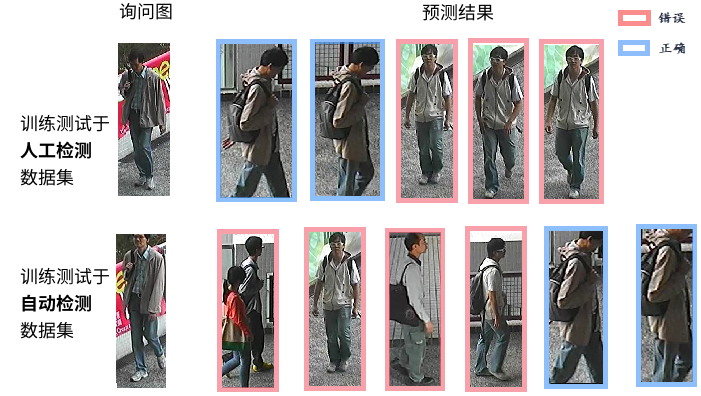
\includegraphics[width=.95\textwidth]{2018-04-18-21-53-15.png}
	\caption{我们的基准模型在手工标注的数据集和行人检测器自动检测的数据集上的典型样例} \label{fig:label2det}
\end{figure}

由此可见需要加入多尺度结构先验,使得模型聚焦于具有鉴别力的区域,才能获得鲁棒而紧凑的行人特征表示。
行人再识别可以看作将不同视角的图片映射到同一个特征空间,从而方便在统一的特征空间中进行比较。在传统的工作中,通常直接使用深度神经网络的最后一层定义统一的特征空间。
但是想要应对各种变化,Yu \etal \cite{yu2017devil}提出中层属性特征与高层语义特征十分重要。
与Yu \etal 工作不同的是,我们
通过注意力机制,抽取、凝练中层属性特征中的重要信息,然后与高层语义表示融合。
我们提出的模型在网络结构上引入先验,从而融合高层语义特征和中层属性特征。
模型包含两个模块:\textbf{(1)、}基于注意力机制的多尺度属性特征提取模块;\textbf{(2)、}特征融合与度量学习模块。

\section{框架设计及算法实现}

\subsection{多尺度属性特征提取模块}

对于特征融合模块,我们对中层特征采用合适的池化方式,然后与最后的语义表示通过拼接的方式形成最终的特征表示。这样的策略,从前向传播的角度看,保证了最终的表示有效包含中层属性信息;从反向传播的角度看,保证了监督信息有效反传更新中层特征,从而学到具有鉴别力的表示。基础的骨架网络也可以采用卷积神经网络结构,比如残差神经网络(ResNet)\cite{he2016identity}、Inception网络\cite{szegedy2015going}、Squeeze \& Extraction网络\cite{hu2017senet}等。

对于行人再识别任务,我们采用在ImageNet上预训练好的ResNet-50模型。
该模型采用全卷积的架构,即所有的参数层都可用卷积层实现。
大量的前人工作直接对最后一层卷积层(res5c)的特征进行全局池化,获得图像的表示$x_4$。
由于在环境、姿态、视角的变化,使用全局特征往往不能很好地鉴别不同的行人,所以
我们同时使用中间层特征来补充$x_4$。
考虑到行人再识别中,姿态的多变性会导致严重的空间失配,图像的空间信息不是很可靠,简单地池化拼接中层属性特征反而会引入背景噪声,造成性能下降,
这一点我们在CUHK03检测数据集上得到了验证。
于是基于目前在ImageNet上效果最好的模型所采用的注意力机制\cite{hu2017senet},我们采用通道层面的注意力机制,在基本不增加计算复杂度的情况下,使得最终的特征更为鲁棒。

\begin{figure}
	\centering
	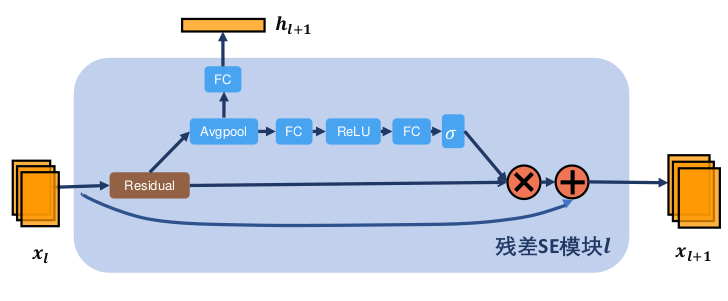
\includegraphics[width=.9\textwidth]{fig/2018-05-11-16-53-10.png}
	\caption{我们提出的残差SE模块}
\end{figure}

\begin{figure}
	\centering
	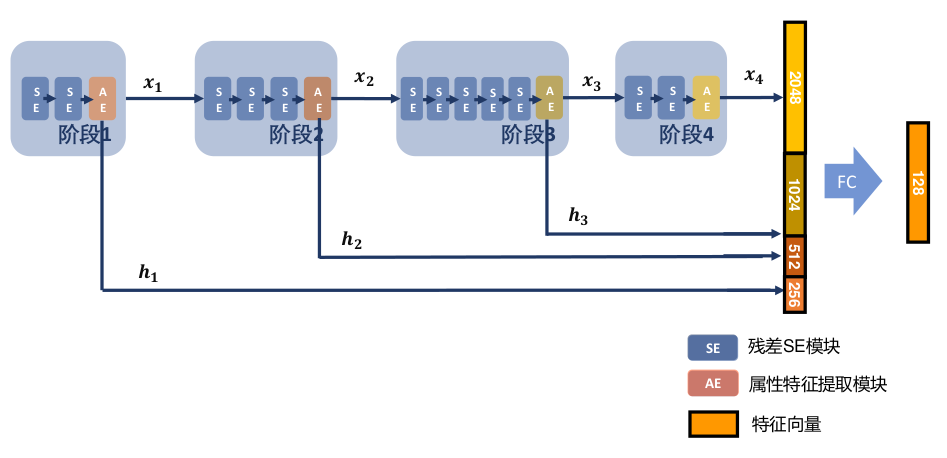
\includegraphics[width=.9\textwidth]{fig/2018-05-11-16-54-07.png}
	\caption{总体框架}
\end{figure}

% \misscite Resource Aware Person Re-identification across Multiple Resolutions
% \begin{figure}
% 	\centering 
% 	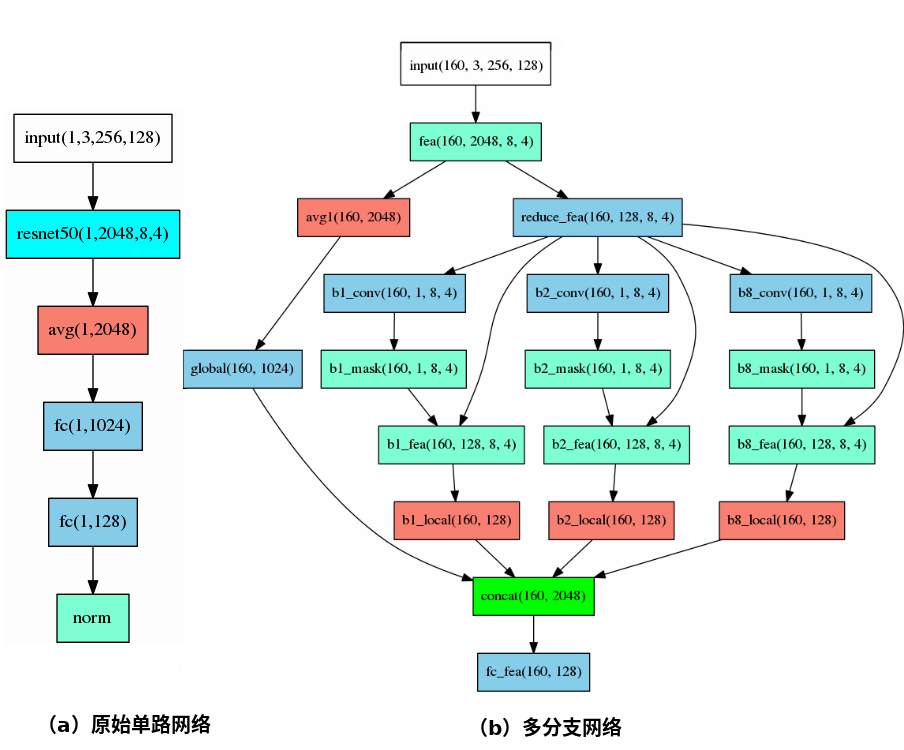
\includegraphics[width=.95\textwidth]{branch.png} 
% 	\caption{多分支模型}
% \end{figure}

计算量
注意力机制

\subsection{特征融合与度量学习模块}

各种特征融合函数
度量学习

\section{实验设计和结果}

\subsection{数据集统计信息与评估协议}

我们提出的算法在六个流行数据集里训练和评测,这六个数据集分别是CUHK03\misscite、CUHK01、ViPeR、PRID450s、prid2011 和i-LIDS。表\ref{table:dataset}列出了各个数据集的ID分布情况和数据规模,以及在实验中训练集和测试集的分布。其中CUHK03数据集提供了两个版本的数据集,分别是由人工标注行人边框的数据和行人检测器自动生成边框的数据集,该数据集包含1360个行人,13164张行人图像,平均每个行人拥有约10 张图像,从两个监控视角里分别采集5张图像,我们在两个数据集上都做了实验,并会报道实验结果。CUHK01数据集包含971 个行人,3884 张行人图像,平均每个行人包含4 张图像,以往工作分别在100 个测试身份和485个测试身份两种训练策略里有相应的实验报告,为了和它们对比,我们在两种策略下也做了相应的实验,并会汇报结果。ViPeR 和PRID450s 是两个相对较小的数据集,在单个视角里每个行人仅仅拥有一张图像。i-LIDS 数据集由在机场到达大厅收集的视频监控构建的,包含119个行人479张图像。PRID2011 包含从两个固定摄像头里捕捉到行人图像,其中一个视角,记作A,包含385个行人的图像,另一个视角,记作B,包含749个行人的图像,两个摄像头有200个行人的重合图像。按照以往工作的测试策略,我们使用每个视角共有的100个行人身份作为训练集,余下的100个行人身份用作测试,测试时,100张来自视角A 的行人图像做为查询图像,来自视角B的100张相同身份的行人图像和剩下的549张行人图像作为搜索库。为了衡量我们提出的SC-PPMN算法性能,并和当前其他相关算法进行比较,我们采用所谓的累积匹配因子(Cumulative Matching Characteristics,CMC),该指标衡量了行人检索性能的优劣,也就是说,给定某一视角下的行人图像作为查询图像,CMC衡量了从样本库里召回的正确样本排在查询列表前面的准确率。
\begin{table}
	\centering
	%\scalebox{0.9}{
	\caption{数据集分布和实验设置。}
	\begin{tabular}{c|cccccc}
		\toprule
		Dataset    & CUHK03\misscite & CUHK01  & VIPeR & PRID450s & i-LIDS & PRID2011 \\
		\hline
		identities & 1360            & 971     & 632   & 450      & 119    & 385/749  \\
		images     & 13164           & 3884    & 1264  & 900      & 479    & 1134     \\
		views      & 2               & 2       & 2     & 2        & 2      & 2        \\
		train IDs  & 1160            & 871;485 & 316   & 225      & 59     & 100      \\
		test IDs   & 100             & 100;486 & 316   & 225      & 59     & 100      \\
		\bottomrule
	\end{tabular}
	%}
	\label{table:dataset}
\end{table}

\subsection{实验结果和比较}

\begin{table}
	\centering
	\caption{在数据集CUHK03上的性能比对。表中列出了CMC(\%)指标在rank-1,rank-5和 rank-10 的结果。}
	% \scalebox{0.95}{
	\begin{tabular}{c|ccc|ccc}
		\toprule
		\multirow{2}*{Methods}               &
		\multicolumn{3}{c|}{labelled CUHK03} &
		\multicolumn{3}{c}{detected CUHK03}                                                                                                        \\
		\cline{2-7}
		\cline{2-7}
		                                     & r=1            & r=5            & r=10           & r=1            & r=5            & r=10           \\ \hline
		KISSME                               & 14.17          & 37.46          & 52.20          & 11.70          & 33.45          & 45.69          \\
		LMNN                                 & 7.29           & 19.64          & 30.74          & 6.25           & 17.87          & 26.60          \\
		LSSCDL                               & 57.00          & -              & -              & 51.20          & -              & -              \\
		LOMO+LSTM                            & -              & -              & -              & 57.30          & 80.10          & 88.30          \\
		LOMO+XQDA                            & 52.20          & 82.23          & 92.14          & 46.25          & 78.90          & 88.55          \\ \hline
		\hline
		FPNN                                 & 20.65          & 50.94          & 67.01          & 19.89          & 49.41          & -              \\
		ImprovedDL                           & 54.74          & 86.50          & 93.88          & 44.96          & 76.01          & 81.85          \\
		PIE(R)+Kissme                        & -              & -              & -              & 67.10          & 92.20          & 96.60          \\
		SICIR                                & -              & -              & -              & 52.17          & -              & -              \\
		DCSL (no hnm)                        & 78.60          & 97.76          & 99.30          & -              & -              & -              \\
		DCSL (hnm)                           & 80.20          & 97.73          & 99.17          & -              & -              & -              \\
		MTDnet                               & 74.68          & 95.99          & 97.47          & -              & -              & -              \\
		JLML                                 & 83.20          & 98.00          & 99.40          & 80.60          & \textbf{96.90} & \textbf{98.70} \\ \hline
		SC-PPMN (no hnm)                     & 83.20          & 97.50          & 99.25          & 77.60          & 96.10          & 98.60          \\
		SC-PPMN (hnm)                        & \textbf{85.50} & \textbf{98.20} & \textbf{99.50} & \textbf{80.63} & 95.62          & 98.07          \\
		\bottomrule
	\end{tabular}

	\label{table:CUHK03}
\end{table}

\section{本章小结}

% -------------------------------------------------------------------------
\chapter{基于对比中心损失的度量学习}
% -------------------------------------------------------------------------

\section{问题描述}

在早期的文献中,度量学习的目标是学习一个相似性函数。通常采用马氏距离
$\norm{\vx_1 - \vx_2}_\mM=
\sqrt{(\vx_1-\vx_2)^T \mM (\vx_1 - \vx_2) }$
作为相似性度量,学习其中的半正定矩阵$\mM$。
但是在最近的文献中,往往使用神经网络自动学习深度嵌入特征$\vx_1, \vx_2$,而使用最简单的距离度量---欧式距离。
通过在欧式空间中设计
带有间隔(margin)损失函数
直接学习行人图片在欧式度量嵌入空间中的
特征表示。
典型的损失函数包括对比损失、三元组损失,
他们都在欧式度量空间中定义了直观的损失函数,使用欧氏距离作为度量,深度网络作为核函数,端到端地学习整体非线性度量函数。

从是否给每个类别创建模板的角度,损失函数可以分为基于模板的损失和基于实例的损失。
从度量函数的角度,损失函数可以分为基于KL散度的损失和基于欧式间隔的损失。(虽然KL散度严格来说不属于度量函数,因为它不具有对称性。但它却是广泛用于表征两个概率分布之间的距离。)
% 比如Zheng?使用Logistic损失函数对“同一行人的类内距离小于不同行人的类间距离”这一事件的概率建模,得到了PRDC模型。
% 图是怎么来的。。。
% 可以方到研究方法里



每一种损失都有各自的优缺点,如图~\ref{fig:losses}所示,中心损失虽然成功学到了每个类别的中心,
但是由于区分每个类别的难易程度是不一样,因此部分类心很容易与临近的类心混淆;
由于每个类别内部样本的差异性也是不一样的,因此部分类心处于该类样本的边缘,容易与临近类别混淆。
交叉损失的分类器权重被视为类心向量与样本特征向量共同嵌入到2维空间可视化,显然每个特征向量被分到了对应类别中心定义的最优分界平面内部的区域,但是这样的特征向量只能用于封闭环境的分类问题,无法适应开放环境的再识别问题。三元组损失虽然通过样本级别的信息成功为不同的类别拉开了一定的距离,但是类内的散度较大。

\begin{figure}
	\centering
	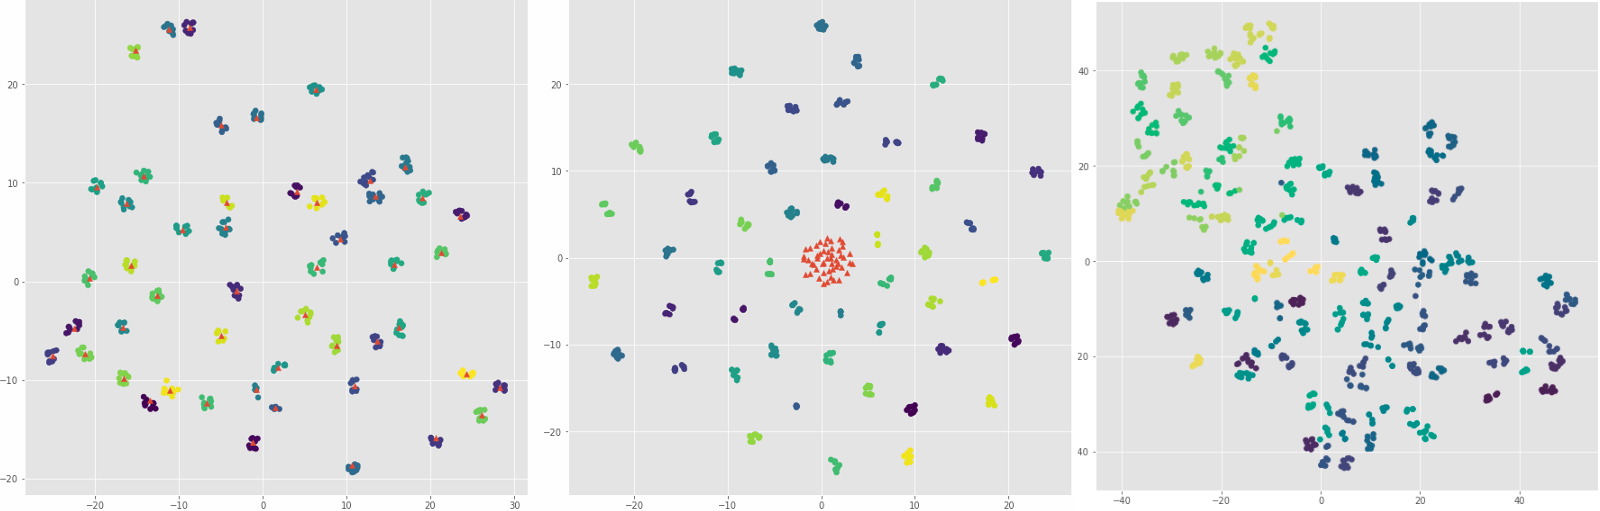
\includegraphics[width=.95\textwidth]{losses.png}
	\caption{三种损失函数监督的验证集特征向量和中心向量在2维平面上降维可视化,使用CUHK03数据集和各损失的基准模型得到}
	\label{fig:losses}
\end{figure}

三元组损失的缺点可以进一步在图~\ref{fig:tsne}中观察到,尽管验证集上的类内内散度已经很小了,但是在测试集上由于有的类别类内散度较大,存在一些样本容易和临近的类别混淆。就是这样的一些样本造成了性能指标的下降。

\begin{figure}
	\centering
	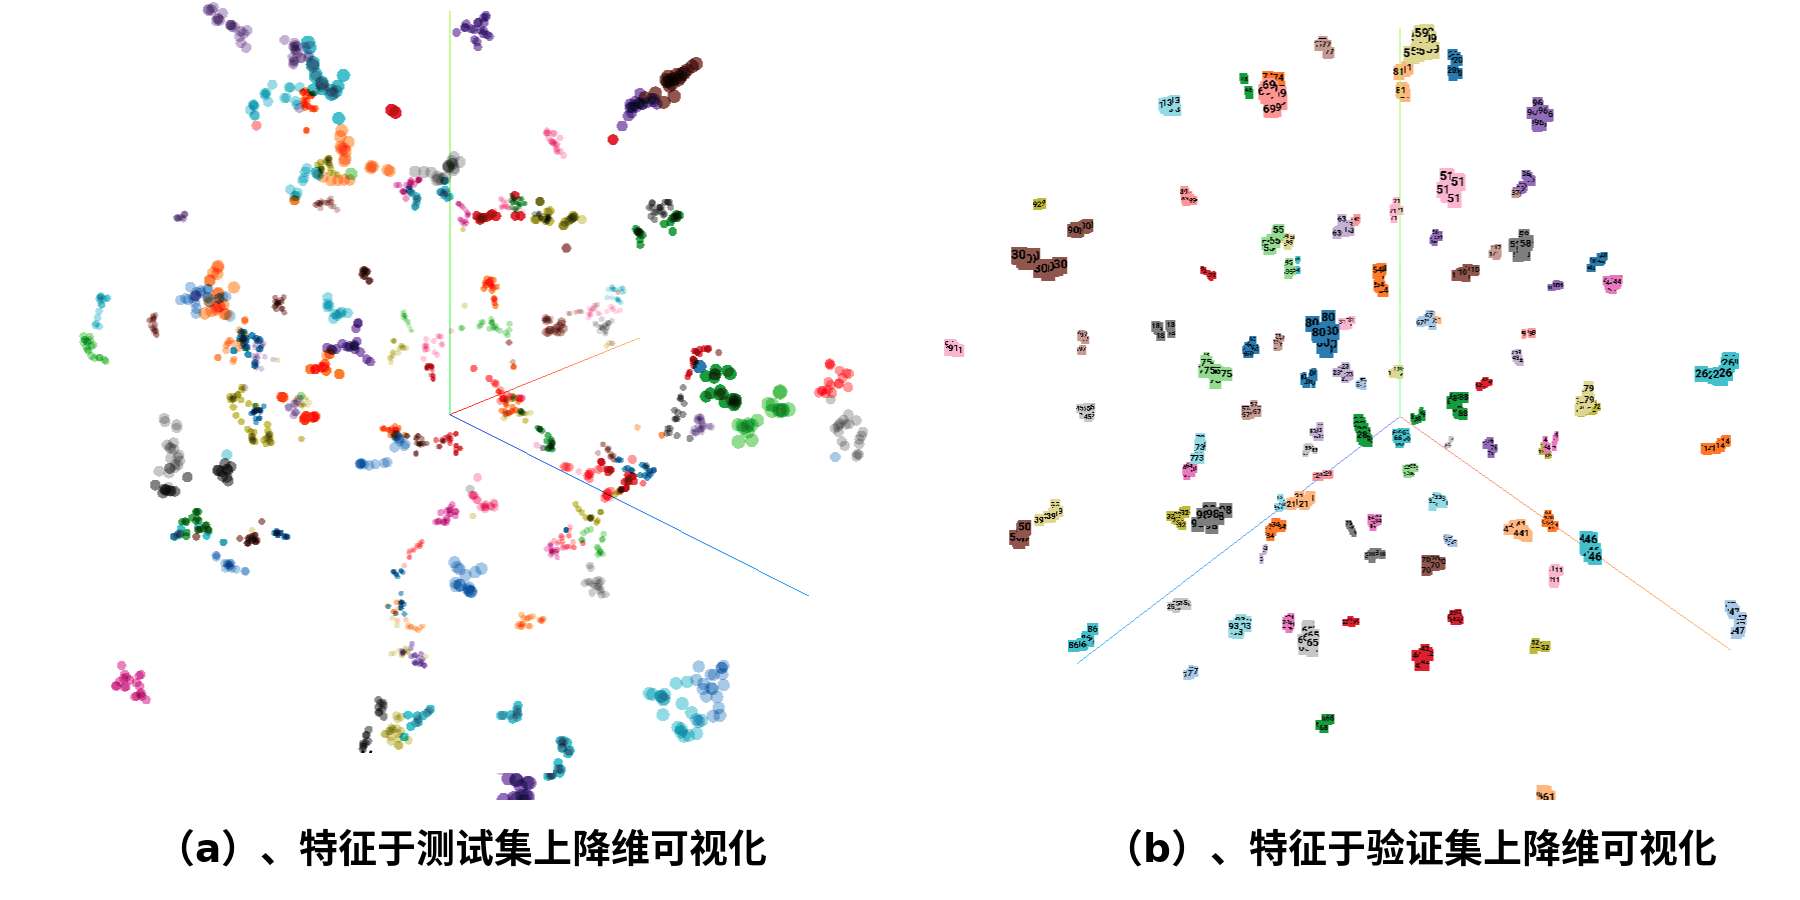
\includegraphics[width=.95\textwidth]{tsne.png}
	\caption{三元组损失在3维空间降维可视化,使用CUHK03数据集和我们的基准模型得到}
	\label{fig:tsne}
\end{figure}

\section{研究方法}

\section{结果验证和分析}

% -------------------------------------------------------------------------
\chapter{结论与展望}
% -------------------------------------------------------------------------

\section{结论}

\section{论文中出现的问题及思考}

\section{展望}

% \bibliographystyle{assets/gbt7714-2005}
% {
\printbibliography[heading=chapbib]
% }